% The Clever Algorithms Project: http://www.CleverAlgorithms.com
% (c) Copyright 2013 Jason Brownlee. Some Rights Reserved. 
% This work is licensed under a Creative Commons Attribution-Noncommercial-Share Alike 2.5 Australia License.


% Name
% The algorithm name defines the canonical name used to refer to the technique, in addition to common aliases, abbreviations, and acronyms. The name is used in terms of the heading and sub-headings of an algorithm description.
\section{Nelder-Mead Method} 
\label{sec:neldermead}
\index{Nelder-Mead Method}
\index{Simplex Algorithm}
\index{Amoeba Algorithm}

% other names
% What is the canonical name and common aliases for a technique?
% What are the common abbreviations and acronyms for a technique?
\emph{Nelder-Mead Method, Downhill Simplex Method, Simplex Method, Amoeba Algorithm.}

% Taxonomy: Lineage and locality
\subsection{Taxonomy}
% To what fields of study does a technique belong?
The Nelder-Mead Method is an optimization algorithm for multidimensional nonlinear unconstrained functions.
It is a Direct Search Method in that it does not use a function gradient during the procedure. It is a Pattern Search in that it uses a geometric pattern to explore the problem space.
% What are the closely related approaches to a technique?
It is related to other Direct Search optimization methods such as Hooke and Jeeves' Pattern Search that also uses a geometric pattern to optimize an objective function.

% Strategy: Problem solving plan
% The strategy is an abstract description of the computational model. The strategy describes the information processing actions a technique shall take in order to achieve an objective. The strategy provides a logical separation between a computational realization (procedure) and a analogous system (metaphor). A given problem solving strategy may be realized as one of a number specific algorithms or problem solving systems. The strategy description is textual using information processing and algorithmic terminology.
\subsection{Strategy}
% What is the information processing objective of a technique?
The information processing objective of the Nelder-Mead Method is to locate the extremum of a function.
% What is a techniques plan of action?
This is achieved by overlaying a simplex (geometrical pattern) in the domain and iteratively increasing and/or reducing its size until an optimal value is found. The simplex is defined always with $n+1$ vertices, where $n$ is the number of dimensions of the search space (i.e. a triangle for a 2D problem).

The process involves identifying the worst performing point of the complex and replacing it with a point reflected through the centroid (center point) of the remaining points. The simplex can be deformed (adapt itself to the topology of the search space) by expanding away from the worst point, contract along one dimension away from the worst point, or contract on all dimensions towards the best point.

% Heuristics: Usage guidelines
% The heuristics element describe the commonsense, best practice, and demonstrated rules for applying and configuring a parameterized algorithm. The heuristics relate to the technical details of the techniques procedure and data structures for general classes of application (neither specific implementations not specific problem instances). The heuristics are described textually, such as a series of guidelines in a bullet-point structure.
\subsection{Heuristics}
% What are the suggested configurations for a technique?
% What are the guidelines for the application of a technique to a problem instance?

\begin{itemize}
	\item It can be used with multi-dimensional functions (one or more parameters) and with non-linear response surfaces.
	\item It does not use a function derivative meaning that it can be used on non-differentiable functions, discontinuous functions, non-smooth functions, and noisy functions.
	\item As a direct search method it is consider inefficient and slow relative to modern derivative-based methods.
	\item It is dependent on the starting position and can be caught by local optimum in multimodal functions.
	\item The stopping criteria can be a minimum change in the best position. 
	\item The nature of the simplex structure can mean it can get stuck in non-optimal areas of the search space, this is more likely if the size of the initial simplex is too large.
	\item When the method does work (is appropriate for the function being optimized) it has been shown to be fast and robust.
\end{itemize}

% sample script in R
\subsection{Code Listing}
% listing
Listing~\ref{stats_nelder_mead} provides a code listing of the Nelder-Mead method in R solving a two-dimensional nonlinear optimization function. Figure~\ref{plot:nelder_mead_result} provides a plot of the test problem with the located minimum highlighted.

% algorithm and package
The example uses the \texttt{optim()} function in the \texttt{stats} core package configured to use the ``Nelder-Mead'' method \cite{RDCT2011a}. The example uses the algorithm default parameters of $\alpha=1.0$ (reflection factor), $\beta=0.5$ (contraction factor), and $\gamma=2.0$ (expansion factor). The procedure will stop if there is no improvement from an iteration (change in response is less than the square root of the machines precision). The \texttt{optim()} function is for General-purpose Optimization, for more information on this library type: \texttt{library(help="stats")}, and for more information on the function type: \texttt{?optim}.

% problem
The test problem is the Rosenbrock function in two-dimensions where the optimum is at $x,y=1$. The starting position for the algorithm is taken as a random point $x,y \in [-3,3]$.

\lstinputlisting[firstline=7,language=r,caption={Example of Nelder-Mead in R using the \texttt{optim()} function in the \texttt{stats} core package.}, label=stats_nelder_mead]{../src/algorithms/optimization/stats_nelder_mead.R}

\begin{figure}[htp]
\centering
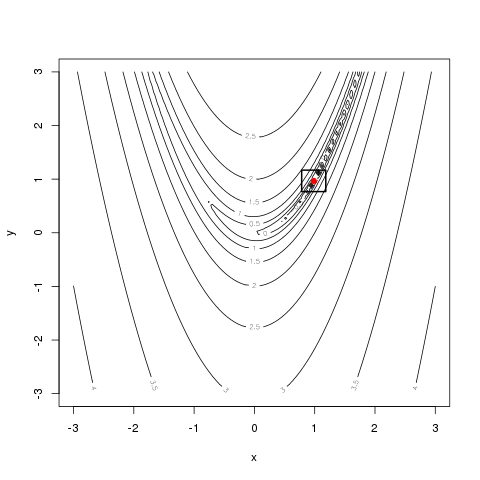
\includegraphics[scale=0.45]{book/a_optimization/nelder_mead_result.png}
\caption{Contour plot of the Rosenbrock function with the located minimum highlighted.}
\label{plot:nelder_mead_result}
\end{figure}

% other packages
The \texttt{gsl} package in the \texttt{multimin()} function provides an implementation of Nelder-Mead algorithm that makes use of the GNU Scientific Library \cite{Hankin2011}.
The \texttt{neldermead} package also provides an implementation of the algorithm \cite{Bihorel2011}.

% References: Deeper understanding
% The references element description includes a listing of both primary sources of information about the technique as well as useful introductory sources for novices to gain a deeper understanding of the theory and application of the technique. The description consists of hand-selected reference material including books, peer reviewed conference papers, journal articles, and potentially websites. A bullet-pointed structure is suggested.
\subsection{References}
% What are the primary sources for a technique?
% What are the suggested reference sources for learning more about a technique?

% primary sources
\subsubsection{Primary Sources}
% seminal
The Simplex optimization algorithm was proposed by Spendley et~al.\ in 1962 that used a simplex and a reflection operator to replace the worst point of the structure \cite{Spendley1962}.
Nelder and Mead extended the method by adding the expansion and contraction rules to the process to increase the rate of convergence in what became known as the Nelder-Mead method \cite{Nelder1965}.

% more info
\subsubsection{More Information}
% study
Lagarias et~al.\ provide a comment of the convergence properties of the Nelder-Mead method on convex one- and two-dimensional problems as well as a careful and complete description of the method clearing up some ambiguous points on its original implementation \cite{Lagarias1998}. Press et~al.\ provide a good summary of the method with sample code in the C programming language \cite{Press2007}. Lewis et~al.\ provide an overview of the procedure and a contemporary perspective on its capabilities in the context of other Direct Search methods \cite{Lewis2000}.
% book
Walters provides a book that focuses on the method which he refers to as Sequential Simplex Optimization \cite{Walters1991}.

% END
